\documentclass[11pt,a4paper]{article}

\usepackage[T1]{fontenc}
\usepackage[utf8]{inputenc}
\usepackage[english]{babel}
\usepackage{amsmath,amssymb}
\usepackage{siunitx}
\usepackage{booktabs}
\usepackage{longtable}
\usepackage{graphicx}
\usepackage{tikz}
\usepackage{listings}
\usepackage{xcolor}
\usepackage[margin=25mm]{geometry}
\usepackage{hyperref}
\hypersetup{colorlinks=true,linkcolor=black,urlcolor=blue,citecolor=black}

\usetikzlibrary{arrows.meta,positioning}

\sisetup{detect-all,per-mode=symbol}

\definecolor{cmt}{rgb}{0.30,0.50,0.30}
\definecolor{kwd}{rgb}{0.10,0.10,0.60}
\definecolor{str}{rgb}{0.60,0.10,0.10}

\lstset{
  basicstyle=\ttfamily\scriptsize,
  commentstyle=\color{cmt}\itshape,
  keywordstyle=\color{kwd}\bfseries,
  stringstyle=\color{str},
  morekeywords={component,nodes,inputs,outputs,parameters,variables,branches,
                equations,events,when,edge,if,else,end,assert,der,Event,true},
  breaklines=true,
  columns=fullflexible,
  frame=single,
  numbers=left,
  numberstyle=\tiny\color{gray},
  showstringspaces=false,
  captionpos=b
}

\newcommand{\Rdson}{R_\mathrm{ds,on}}
\newcommand{\Eon}{E_\mathrm{on}}
\newcommand{\Eoff}{E_\mathrm{off}}
\newcommand{\Err}{E_\mathrm{rr}}
\newcommand{\Tj}{T_\mathrm{j}}
\newcommand{\dd}{\mathrm{d}}

\title{\texttt{pelib.mos\_simple\_2th}\\
       A simplified power MOSFET loss model in Simscape Language}
\author{Documentation}
\date{Revision 1.0}

\begin{document}
\maketitle

\begin{abstract}
This document describes a Simscape Language component for converter-level loss
and junction-temperature estimation of power MOSFETs. The switching transient is
not resolved: the device commutates in one solver step and the switching
energies are taken from single datasheet values, scaled to the operating point.
Conduction and switching losses are separated between the transistor die and the
diode die and delivered to two thermal ports. The model follows the same
structure as the corresponding IGBT model, from which it differs in the
treatment of the bidirectional channel, in the attribution of the third-quadrant
losses, and in the option of a single junction when the diode is intrinsic.
\end{abstract}

\tableofcontents

% ======================================================================
\section{Modelling assumptions}

The model answers one question: how much power is dissipated, and where. It does
not answer any question about the shape of the transient. The assumptions are
listed explicitly, because most of the criticism that can be made of the model
is already contained in them.

\begin{enumerate}
\item \textbf{The switching transient is not resolved.} There is no $\dd i/\dd t$,
      no voltage overshoot, no gate-loop dynamics. The channel conductance
      changes discontinuously with the gate command. This is deliberate: an
      instantaneous transition contributes exactly zero crossover energy to the
      conduction term $v\,i_\mathrm{ch}$, which leaves the switching energies
      entirely to the event mechanism of
      Section~\ref{sec:switching} and avoids double counting.
\item \textbf{Switching energies come from a single reference point.} One value
      of $\Eon$, $\Eoff$ and $\Err$ at $(I_\mathrm{ref},V_\mathrm{ref})$, scaled
      by a power law. The error grows away from the reference point.
\item \textbf{No temperature dependence of the switching energies}, and none of
      the diode forward characteristic. For SiC this is a minor omission, since
      $\Eon$ and $\Eoff$ are nearly temperature independent; for silicon it is
      not, and the parameters must be taken at the maximum expected junction
      temperature.
\item \textbf{Electrothermal feedback is optional and limited to $\Rdson$.}
      With $\alpha_R=0$ the model is a pure feed-forward loss calculator and the
      electrical solution is independent of the thermal network. This is the
      default, and it is the configuration intended for nominal-value
      dimensioning.
\item \textbf{The gate command is a clean logic signal with dead time.} Because
      the channel switches discontinuously, cross-conduction is prevented by the
      external modulator, not by the device model.
\end{enumerate}

% ======================================================================
\section{Interface}

\subsection{Ports}

\begin{table}[h]
\centering
\begin{tabular}{llp{85mm}}
\toprule
Port & Type & Meaning \\
\midrule
\texttt{p}  & electrical         & Drain \\
\texttt{n}  & electrical         & Source \\
\texttt{G}  & physical signal in & Gate command, $0$ or $1$ \\
\texttt{Ht} & thermal            & MOSFET die \\
\texttt{Hd} & thermal            & Diode die \\
\texttt{Pt} & physical signal out& Transistor dissipated power, \si{\watt} \\
\texttt{Pd} & physical signal out& Diode dissipated power, \si{\watt} \\
\bottomrule
\end{tabular}
\caption{Component interface. The port-side annotation in the \texttt{.ssc}
source accepts only \texttt{left} and \texttt{right}.}
\end{table}

\subsection{Parameters}

\begin{longtable}{lllp{62mm}}
\toprule
Name & Default & Unit & Meaning \\
\midrule
\endhead
\texttt{Rds\_on}  & \num{2.5e-3} & \si{\ohm}   & On-state resistance at \texttt{Tj\_ref} \\
\texttt{alpha\_R} & \num{0}      & \si{\per\kelvin} & Temperature coefficient of $\Rdson$; $0$ disables the feedback \\
\texttt{Tj\_ref}  & \num{398.15} & \si{\kelvin}& Reference junction temperature (\SI{125}{\celsius}) \\
\texttt{Roff}     & \num{1e7}    & \si{\ohm}   & Off-state resistance \\
\texttt{Vf}       & \num{1.0}    & \si{\volt}  & Diode knee voltage \\
\texttt{Rd}       & \num{2.5e-3} & \si{\ohm}   & Diode differential resistance \\
\texttt{two\_die} & \num{1}      & --          & $1$: diode losses to \texttt{Hd}; $0$: to \texttt{Ht} \\
\texttt{Eon\_ref} & \num{12e-3}  & \si{\joule} & Turn-on energy at the reference point \\
\texttt{Eoff\_ref}& \num{8e-3}   & \si{\joule} & Turn-off energy at the reference point \\
\texttt{Err\_ref} & \num{0.5e-3} & \si{\joule} & Diode recovery energy at the reference point \\
\texttt{Iref}     & \num{600}    & \si{\ampere}& Reference current of the energy data \\
\texttt{Vref}     & \num{600}    & \si{\volt}  & Reference dc voltage of the energy data \\
\texttt{ki}       & \num{1}      & --          & Current exponent \\
\texttt{kv}       & \num{1}      & --          & Voltage exponent \\
\texttt{Vth\_off} & \num{50}     & \si{\volt}  & Turn-off and recovery detection threshold \\
\texttt{Vth\_on}  & \num{25}     & \si{\volt}  & Turn-on detection threshold \\
\texttt{V\_sm}    & \num{10}     & \si{\volt}  & Smoothing width of the blocking indicator \\
\texttt{tau\_s}   & \num{100e-9} & \si{\second}& Sample-and-hold time constant \\
\texttt{tau\_v}   & \num{10e-6}  & \si{\second}& Blocking-voltage estimator time constant \\
\texttt{tau\_p}   & \num{50e-6}  & \si{\second}& Energy-to-power lag time constant \\
\texttt{i\_eps}, \texttt{v\_eps} & \num{1e-3} & \si{\ampere}, \si{\volt} & Smoothing constants \\
\bottomrule
\caption{Parameters. The defaults are placeholders representative of a
\SI{1200}{\volt}/\SI{600}{\ampere} SiC MOSFET half-bridge module at
\SI{125}{\celsius}; they are not taken from a specific datasheet.}
\end{longtable}

% ======================================================================
\section{Conduction}

\subsection{Two parallel branches}

Let $v = v_\mathrm{p} - v_\mathrm{n}$ be the drain-source voltage and $i$ the
current entering the drain. Channel and diode are written as two branches across
the same voltage, not as two alternative operating modes:
\begin{align}
  i_\mathrm{ch} &= G_\mathrm{ch}\,v,
  & G_\mathrm{ch} &=
  \begin{cases}
    1/R_\mathrm{ds} & G > 0.5\\[2pt]
    1/R_\mathrm{off}& \text{otherwise}
  \end{cases}
  \label{eq:chan}\\[4pt]
  i_\mathrm{d} &= \frac{1}{R_\mathrm{d}}\,
                  \big[\,-v - V_\mathrm{f}\,\big]^{+},
  \label{eq:diode}\\[4pt]
  i &= i_\mathrm{ch} - i_\mathrm{d}.
\end{align}
The positive part is regularised as
\begin{equation}
  [x]^{+} \;\simeq\; \frac{x + \sqrt{x^{2} + \varepsilon^{2}}}{2},
  \label{eq:softmax}
\end{equation}
which removes the kink at $x = 0$ at the cost of a residual current
$\varepsilon/(2R_\mathrm{d})$ at zero overdrive; with the default values this is
\SI{0.2}{\ampere}, three orders of magnitude below the rated current. For
$v \ll -V_\mathrm{f}$ the two terms of \eqref{eq:softmax} cancel to
$\varepsilon^{2}/(4|x|)$, so the blocking leakage is negligible and, more
importantly, bounded.

This formulation is the main structural difference with respect to the IGBT
model. In the third quadrant with the gate high, both branches are active
simultaneously and the current splits according to their characteristics:
\begin{equation}
  \frac{i_\mathrm{d}}{|i|} \;\ne\; 0
  \quad\text{only if}\quad
  R_\mathrm{ds}\,|i| > V_\mathrm{f}.
\end{equation}
With $R_\mathrm{ds} = \SI{2.5}{\milli\ohm}$ and $V_\mathrm{f} = \SI{1}{\volt}$
the diode starts to take a share above \SI{400}{\ampere}, which is the physical
behaviour of a synchronously driven device and does not need to be imposed.

\subsection{Loss attribution}

\begin{equation}
  P_\mathrm{c,t} = v\,i_\mathrm{ch} = \frac{v^{2}}{R_\mathrm{ds}} = R_\mathrm{ds} i_\mathrm{ch}^{2},
  \qquad
  P_\mathrm{c,d} = -v\,i_\mathrm{d} .
\end{equation}
Both are non-negative by construction, in either quadrant. The channel loss is
charged to \texttt{Ht} regardless of the sign of the current: synchronous
rectification is a transistor loss, not a diode loss. Note also that the
transistor conduction loss is quadratic in current, whereas the IGBT model gives
the affine form $V_\mathrm{ce,sat} i + R_\mathrm{on} i^{2}$. At partial load the
MOSFET is therefore comparatively better, and a dimensioning based on the rated
point alone will be conservative rather than optimistic.

\subsection{Temperature dependence of \texorpdfstring{$\Rdson$}{Rds,on}}

Setting $\alpha_R \ne 0$ enables
\begin{equation}
  R_\mathrm{ds} = \Rdson \Big[\,0.2 + \big[\,x_R - 0.2\,\big]^{+}\,\Big],
  \qquad
  x_R = 1 + \alpha_R\,(T_{\mathrm{Ht}} - \Tj^\mathrm{ref}),
\end{equation}
with the positive part again regularised as in \eqref{eq:softmax}. The floor at
$0.2\,\Rdson$ keeps the resistance positive if the thermal network is
initialised far below the operating temperature; without it, a coefficient of
\SI{0.006}{\per\kelvin} would produce a negative resistance below
\SI{-106}{\celsius}, which is outside any physical range but well inside the
range a solver can visit during initialisation.

Enabling this term closes an algebraic loop between the electrical solution and
the thermal network. The loop is well posed and Simscape handles it, but it
enlarges the nonlinear system and it makes the losses depend on the initial
temperature of the Foster network. For a dimensioning at nominal values the
recommended configuration is $\alpha_R = 0$ with $\Rdson$ read at the maximum
junction temperature. Representative coefficients around \SI{125}{\celsius} are
\SIrange{0.005}{0.008}{\per\kelvin} for SiC and
\SIrange{0.008}{0.012}{\per\kelvin} for silicon superjunction devices.

% ======================================================================
\section{Switching losses}\label{sec:switching}

\subsection{Scaling law}

Each event adds an energy
\begin{equation}
  E = E_\mathrm{ref}
      \left(\frac{I}{I_\mathrm{ref}}\right)^{k_i}
      \left(\frac{V_\mathrm{bl}}{V_\mathrm{ref}}\right)^{k_v},
  \label{eq:scaling}
\end{equation}
where $k_i = k_v = 1$ reproduces the usual bilinear scaling. The power-law form
is preferred to a polynomial fit because it remains positive for any argument,
which matters when the solver evaluates the expression during a rejected step.

$V_\mathrm{bl}$ is not the instantaneous terminal voltage, which at the
detection instant is only $V_\mathrm{th}$. It is a held estimate of the blocking
voltage, obtained by tracking $v$ only while the device is blocking:
\begin{equation}
  \tau_v\,\dot V_\mathrm{bl} = h_\mathrm{b}\,(v - V_\mathrm{bl}),
  \qquad
  h_\mathrm{b} = \tfrac{1}{2}\left[1 + \tanh\frac{v - V_\mathrm{th,off}}{V_\mathrm{sm}}\right].
\end{equation}
The $\tanh$ indicator is used instead of a conditional expression so that no
additional zero crossing is generated. With $\tau_v \ll$ the blocking interval,
$V_\mathrm{bl}$ converges to the dc-link voltage; when the voltage collapses,
$h_\mathrm{b} \to 0$ and the value is frozen and available at the event.

\subsection{Event detection}

The switching instants are detected on the terminal voltage rather than on the
gate command, because the terminal voltage is what distinguishes a commutation
that actually happened from one that was only commanded.

\begin{table}[h]
\centering
\begin{tabular}{lllp{45mm}}
\toprule
Event & Trigger & Energy & Current \\
\midrule
Turn-on   & $v$ falls below $V_\mathrm{th,on}$  & $G\cdot\Eon$ & terminal current at the event \\
Turn-off  & $v$ rises above $V_\mathrm{th,off}$ & $\Eoff$      & $i_\mathrm{th}$, held \\
Recovery  & $v$ rises above $V_\mathrm{th,off}$ & $\Err$       & $i_\mathrm{dh}$, held \\
\bottomrule
\end{tabular}
\caption{Event table. Two distinct thresholds provide hysteresis and prevent
chattering when the terminal voltage lingers near the detection level.}
\end{table}

The factor $G$ on the turn-on energy suppresses the spurious detection produced
during the dead time, when the voltage collapses because the diode of this same
device starts to conduct: there the gate is low and the term vanishes. A turn-on
that occurs while the diode is already conducting produces no down-crossing at
all, since $v$ is already negative; a zero-voltage turn-on therefore costs
nothing, without any special-case logic.

At the turn-on event the current is sampled directly, because the commutation
from the complementary device is complete by the time the voltage has fallen
below $V_\mathrm{th,on}$. At the turn-off event this is not true: the current has
already left the device, and a held value is required.

\subsection{Sample-and-hold states}

Turn-off and reverse recovery share a single trigger, because the terminal
voltage rises in two distinct situations: when this transistor turns off, and
when the complementary switch turns on and reverse-biases this diode. Both
energies are evaluated at every up-crossing, and the correct one is selected by
two tracking states rather than by a mode test:
\begin{align}
  \tau_s\,\dot i_\mathrm{th} &= G\,\big([\,i_\mathrm{ch}\,]^{+} - i_\mathrm{th}\big),
  \label{eq:ith}\\
  \tau_s\,\dot i_\mathrm{dh} &= i_\mathrm{d} - i_\mathrm{dh}.
  \label{eq:idh}
\end{align}
Equation~\eqref{eq:ith} tracks the \emph{positive part} of the channel current
while the gate is high and holds when it is low. Two consequences follow. In
first-quadrant conduction, $i_\mathrm{th}$ equals the load current and is frozen
at the value it had immediately before the gate went low, which is exactly what
$\Eoff$ requires. In synchronous rectification the channel current is negative,
$[\,i_\mathrm{ch}\,]^{+} \to 0$, and the state decays to zero: the subsequent
up-crossing produces $\Eoff = 0$, which is correct, since turning the channel
off into its own conducting diode is a soft transition.

Equation~\eqref{eq:idh} tracks the diode current unconditionally. While the
channel shunts the diode, $i_\mathrm{d}\simeq 0$ and the state follows it down;
during the dead time the diode takes the full load current and the state
recovers it. Hence exactly one $\Err$ event per switching period, in the half
period in which the diode actually conducts, and $\Err = 0$ in the other half.

The choice of $\tau_s$ is the one real constraint of the scheme:
\begin{equation}
  \tau_s \ll t_\mathrm{dead},
\end{equation}
otherwise $i_\mathrm{dh}$ does not reach the load current before the recovery
event and $\Err$ is underestimated. The default \SI{100}{\nano\second} against a
dead time of \SIrange{1}{2}{\micro\second} gives ten to twenty time constants,
i.e.\ an error below \SI{0.01}{\percent}. Reducing $\tau_s$ further only adds a
fast mode to the system without improving the result.

\subsection{Sequence over one switching period}

Figure~\ref{fig:timing} shows the two half periods of a leg operating with
positive and with negative load current, and the resulting event attribution.

\begin{figure}[h]
\centering
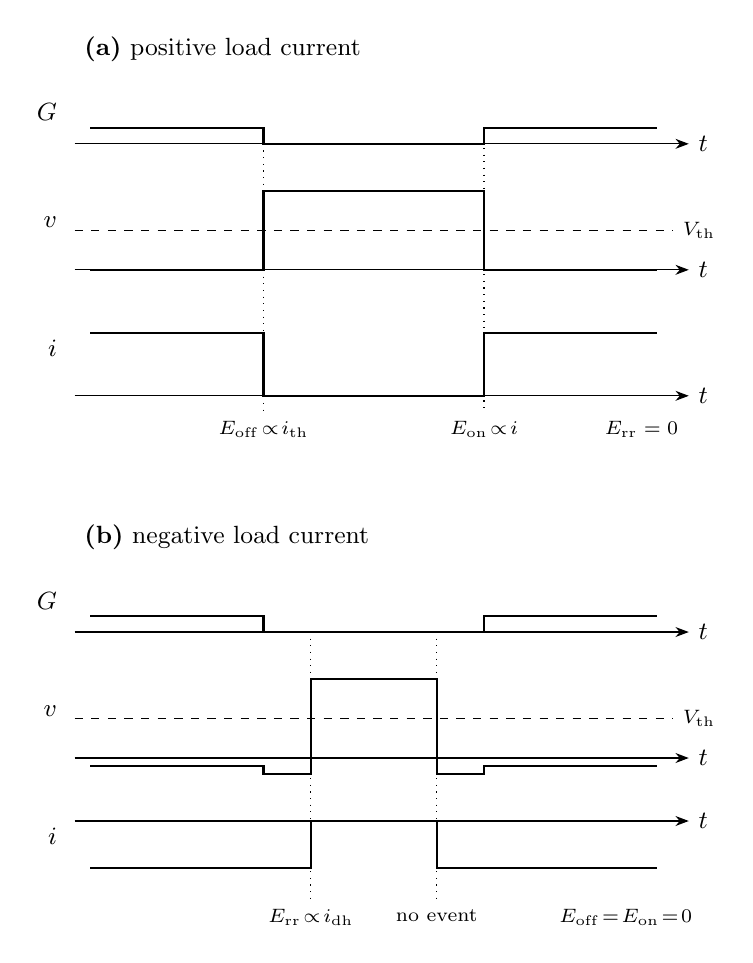
\begin{tikzpicture}[x=1mm,y=1mm,>=Stealth,line width=0.4pt]

% ---------- positive current ----------
\node[anchor=west] at (0,44) {\small\textbf{(a)} positive load current};

\draw[->] (0,32) -- (78,32) node[right] {\small $t$};
\node[anchor=east] at (-1,36) {\small $G$};
\draw[thick] (2,34) -- (24,34) -- (24,32) -- (52,32) -- (52,34) -- (74,34);

\draw[->] (0,16) -- (78,16) node[right] {\small $t$};
\node[anchor=east] at (-1,22) {\small $v$};
\draw[thick] (2,16) -- (24,16) -- (24,26) -- (52,26) -- (52,16) -- (74,16);
\draw[dashed] (0,21) -- (76,21) node[right,font=\scriptsize] {$V_\mathrm{th}$};

\draw[->] (0,0) -- (78,0) node[right] {\small $t$};
\node[anchor=east] at (-1,6) {\small $i$};
\draw[thick] (2,8) -- (24,8) -- (24,0) -- (52,0) -- (52,8) -- (74,8);

\draw[dotted] (24,32) -- (24,-2);
\draw[dotted] (52,34) -- (52,-2);
\node[font=\scriptsize,anchor=north] at (24,-2) {$\Eoff\!\propto\! i_\mathrm{th}$};
\node[font=\scriptsize,anchor=north] at (52,-2) {$\Eon\!\propto\! i$};
\node[font=\scriptsize,anchor=north] at (72,-2) {$\Err = 0$};

% ---------- negative current ----------
\begin{scope}[yshift=-62mm]
\node[anchor=west] at (0,44) {\small\textbf{(b)} negative load current};

\draw[->] (0,32) -- (78,32) node[right] {\small $t$};
\node[anchor=east] at (-1,36) {\small $G$};
\draw[thick] (2,34) -- (24,34) -- (24,32) -- (52,32) -- (52,34) -- (74,34);

\draw[->] (0,16) -- (78,16) node[right] {\small $t$};
\node[anchor=east] at (-1,22) {\small $v$};
\draw[thick] (2,15) -- (24,15) -- (24,14) -- (30,14) -- (30,26) -- (46,26)
             -- (46,14) -- (52,14) -- (52,15) -- (74,15);
\draw[dashed] (0,21) -- (76,21) node[right,font=\scriptsize] {$V_\mathrm{th}$};

\draw[->] (0,8) -- (78,8) node[right] {\small $t$};
\node[anchor=east] at (-1,6) {\small $i$};
\draw[thick] (2,2) -- (30,2) -- (30,8) -- (46,8) -- (46,2) -- (74,2);

\draw[dotted] (30,32) -- (30,-2);
\draw[dotted] (46,32) -- (46,-2);
\node[font=\scriptsize,anchor=north] at (30,-2) {$\Err\!\propto\! i_\mathrm{dh}$};
\node[font=\scriptsize,anchor=north] at (46,-2) {no event};
\node[font=\scriptsize,anchor=north] at (70,-2) {$\Eoff\!=\!\Eon\!=\!0$};
\end{scope}

\end{tikzpicture}
\caption{Attribution of the switching energies. In (a) the channel conducts the
positive load current: the up-crossing of $v$ charges $\Eoff$ with the held
channel current, and the down-crossing charges $\Eon$ with the freshly
commutated terminal current; the diode never conducts, so $i_\mathrm{dh}=0$ and
no recovery energy is produced. In (b) the current is negative: the channel
conducts synchronously, $i_\mathrm{th}$ has decayed to zero, the diode picks up
the current during the dead time and the up-crossing produced by the turn-on of
the complementary switch charges $\Err$ only. Waveforms are schematic; the
dead-time intervals are exaggerated.}
\label{fig:timing}
\end{figure}

% ======================================================================
\section{From energy to power}

The event energies are accumulated in two event variables $E_\mathrm{q}$, which
are piecewise constant and jump at each event. A continuous state follows them
through a first-order lag:
\begin{equation}
  \tau_p\,\dot E_\mathrm{o} = E_\mathrm{q} - E_\mathrm{o},
  \qquad
  P_\mathrm{sw} = \frac{E_\mathrm{q} - E_\mathrm{o}}{\tau_p} = \dot E_\mathrm{o}.
\end{equation}
Since the delivered power is by construction the derivative of $E_\mathrm{o}$,
\begin{equation}
  \int_{0}^{t} P_\mathrm{sw}\,\dd\tau = E_\mathrm{o}(t)
  = E_\mathrm{q}(t) - \tau_p P_\mathrm{sw}(t),
\end{equation}
so the energy is conserved exactly up to the residual $\tau_p P_\mathrm{sw}$,
which is bounded by the largest single event energy and vanishes in the mean.
The lag introduces no bias: it only spreads each pulse over a time $\tau_p$.

The choice of $\tau_p$ follows from two inequalities:
\begin{equation}
  T_\mathrm{sw} \lesssim \tau_p \ll \min_k \tau_{\mathrm{th},k},
\end{equation}
where $\tau_{\mathrm{th},k}$ are the time constants of the Foster network. The
lower bound smooths the pulse train and keeps the solver from tracking a
sequence of impulses; the upper bound guarantees that the thermal response is
not distorted. At \SI{20}{\kilo\hertz} and with a fastest Foster time constant
of the order of \SI{1}{\milli\second}, any $\tau_p$ between \SI{50}{\micro\second}
and \SI{200}{\micro\second} is acceptable.

% ======================================================================
\section{Thermal ports}

\subsection{Sign convention}

The thermal branches are declared as
\begin{center}
\texttt{Qt : Ht.Q -> *;} \qquad \texttt{Qd : Hd.Q -> *;}
\end{center}
so that $Q$ is positive when heat flows into the component. The equations
therefore read
\begin{equation}
  Q_\mathrm{t} = -P_\mathrm{t},
  \qquad
  Q_\mathrm{d} = -P_\mathrm{d},
\end{equation}
with $P_\mathrm{t}$ and $P_\mathrm{d}$ the dissipated powers, also exported as
physical signal outputs for bookkeeping.

\subsection{One die or two}

\begin{equation}
  P_\mathrm{t} = P_\mathrm{c,t} + P_\mathrm{sw,t}
                 + (1 - \nu)\,(P_\mathrm{c,d} + P_\mathrm{sw,d}),
  \qquad
  P_\mathrm{d} = \nu\,(P_\mathrm{c,d} + P_\mathrm{sw,d}),
\end{equation}
where $\nu = \texttt{two\_die} \in \{0,1\}$.

With $\nu = 1$ the diode losses are delivered to \texttt{Hd}. This is the case of
a module carrying a separate antiparallel die, typically a SiC MOSFET with a SiC
Schottky diode, where the two junctions have different $R_\mathrm{th(j-c)}$ and
deserve separate temperatures.

With $\nu = 0$ the diode losses are added to \texttt{Ht} instead. This must be
used whenever the diode is the intrinsic body diode: it is the same die as the
channel, and modelling two independent junctions would be an error rather than a
refinement. Port \texttt{Hd} then carries no heat, but it must still be
connected, for instance to a Thermal Reference or to the same node as
\texttt{Ht}.

A practical consequence: since the body diode of a synchronously driven MOSFET
conducts only during the dead time, its contribution is small, but it is
concentrated on the same junction that already carries the channel loss. The
single-junction configuration is therefore not conservative by accident; it is
simply correct.

% ======================================================================
\section{Parameter extraction}

\begin{itemize}
\item $\Rdson$ at the junction temperature at which the dimensioning is
      performed and at the actual gate voltage. Datasheets normally give
      \SI{25}{\celsius} and \SI{150}{\celsius}; interpolate, and remember that
      the value at \SI{25}{\celsius} is the marketing number, not the design
      number.
\item $V_\mathrm{f}$ and $R_\mathrm{d}$ from the third-quadrant characteristic
      measured with $V_\mathrm{gs}$ at its negative off-state value, not from
      the synchronous-conduction curve, which is the channel and is already
      accounted for by \eqref{eq:chan}.
\item $\Eon$, $\Eoff$ from the energy-versus-current curves at the gate voltage,
      gate resistance and dc voltage of the application. Choose
      $I_\mathrm{ref}$ close to the current at which the converter actually
      operates: with $k_i = 1$ the error of \eqref{eq:scaling} is zero at the
      reference point and grows away from it.
\item $\Err$ from the recovery-energy curve, or from
      $\Err \simeq V_\mathrm{dc} Q_\mathrm{rr}$ when only $Q_\mathrm{rr}$ is
      given. For a Schottky diode the recovered charge is capacitive only: the
      appropriate value is small but not zero.
\end{itemize}

Two remarks specific to MOSFETs:

\begin{enumerate}
\item The datasheet $\Eon$ is measured in a hard-switched double-pulse test and
      already includes the reverse recovery of the complementary diode and the
      discharge of $C_\mathrm{oss}$. Neither must be added again.
\item Under zero-voltage switching the datasheet $\Eon$ is meaningless. If the
      model is used in a resonant, dual-active-bridge or phase-shifted
      converter, $\Eon$ must be replaced by the $C_\mathrm{oss}$ hysteresis
      energy of the device, one to two orders of magnitude smaller. It is worth
      checking, by monitoring \texttt{Pt}, that the model is not detecting
      turn-on events that in the real converter are soft.
\end{enumerate}

% ======================================================================
\section{Limits of validity}

\begin{itemize}
\item No transient waveform information: no $\dd i/\dd t$, no overshoot, no gate
      resistance dependence, no snubber evaluation. For those, a
      switching-dynamics model such as \texttt{mos\_dyn} is required.
\item Energies scaled from one reference point; error grows with distance from
      it, and the linear current law underestimates the curvature of the real
      $E(I)$ characteristic at low current.
\item No temperature dependence of the switching energies or of the diode
      characteristic.
\item Off-state leakage is set by $R_\mathrm{off}$, not by a physical model. At
      \SI{1200}{\volt} the default gives \SI{0.14}{\watt} of spurious blocking
      loss, negligible against the hundreds of watts of a rated device but worth
      remembering if the model is used at very light load.
\item The model relies on external dead time. With zero dead time the recovery
      current is underestimated, and cross-conduction is not prevented by the
      component.
\end{itemize}

% ======================================================================
\section{Suggested verification}

\begin{enumerate}
\item Constant duty cycle and constant load current: compare
      $\overline{P_\mathrm{t}} + \overline{P_\mathrm{d}}$ against the hand
      calculation
      $R_\mathrm{ds} I_\mathrm{rms}^{2} + (\Eon + \Eoff) f_\mathrm{sw}
      (I/I_\mathrm{ref})(V_\mathrm{dc}/V_\mathrm{ref})$.
\item Sweep the sign of the load current and verify that $P_\mathrm{d}$
      collapses in the half period in which the channel conducts synchronously,
      and that $\Eoff$ vanishes there.
\item Set $\nu = 0$ and verify that $P_\mathrm{t}$ gains exactly what
      $P_\mathrm{d}$ loses.
\item If the solver reports scaling problems, add explicit \texttt{nominal}
      values to the energy variables \texttt{Eqt}, \texttt{Eqd}, \texttt{Eot},
      \texttt{Eod}.
\end{enumerate}

% ======================================================================
\appendix
\section{Source listing}

\lstinputlisting[language=Matlab]{mos_simple_2th.ssc}

\end{document}
